\section{Conclusion}
\subsection*{Future work}
\subsubsection{Path position leak}
In HOPR, payments are performed hop-by-hop along a packet’s route.
The incentives break the unlinkability guarantees inherited from the SPHINX packet format as they reveal the identity of the packet origin who transfers those incentives in the channel using their signature. 
\\To solve this problem, HOPR forward incentives next to the packet.
\begin{figure}[H]
    \centering
    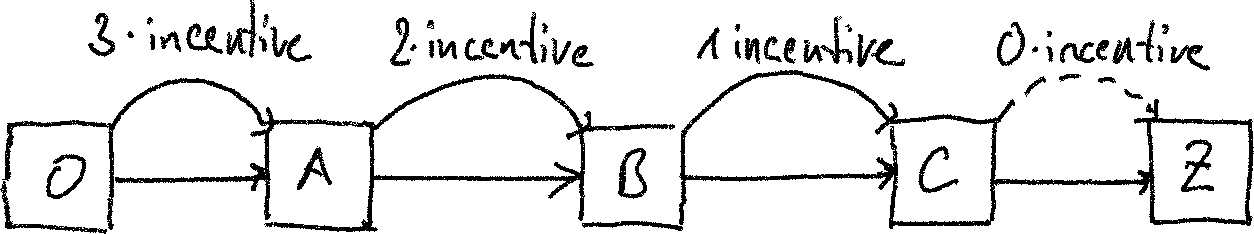
\includegraphics[width=10cm,height=10cm,keepaspectratio]{../whitepaper/images/token_cashflow.png}
    \caption{Incentive flow}
    \label{fig:Incentive flow}
    \end{figure}

    \hspace{-5mm}This however leaks the relayer’s position within the selected path since the value of the ticket is set according to the current relay fee and the number of intermediate hops, 
more precisely $$amount:=\frac{(hops -1)* relayFee}{winProb}$$
This leakage is considered to have a low severity but further research will be conducted on the subject.
